\documentclass{beamer}
\usetheme[
  block=fill,
  background=dark,
  titleformat=smallcaps,
  progressbar=frametitle,
  numbering=none,
]{metropolis}

% Math
\usepackage{amsmath}
\usepackage{amssymb}
\usepackage{stmaryrd}

% Code listing
\usepackage{minted}
\usemintedstyle{monokai}
\newcommand{\icode}[1]{\mintinline{haskell}{#1}}

% Graphics
\usepackage{graphics}
\usepackage{pdfpages}
\graphicspath{{figures/}} % Location of the graphics files

\newcommand\todo[1]{\textcolor{red}{#1}}

%----------------------------------------------------------------------------

\title{AlgoRhythm}
\subtitle{A Library for Algorithmic Music Composition}
\author{Joris ten Tusscher, Cas van der Rest, Orestis Melkonian}
\date{April 5, 2018}
\institute{Universiteit Utrecht}

\begin{document}
	\maketitle
	
	\begin{frame}{Music DSL}
	\todo{music representation (Music, MusicCore, Scale, Chord, etc...}\\
	\todo{music manipulation (transpose, retrograde, time-scale, etc...}\\
	\end{frame}
		
	{\usebackgroundtemplate{%
  	
\includegraphics[width=\paperwidth,height=\paperheight]{no-analysis.png}}
	\begin{frame}{Focus on Generation, Ignore Analysis}
	\end{frame}
	}	
	
	\begin{frame}{Generation}
	\todo{genState, selectors, diatonic improv, etc...}
	\end{frame}
	
	\begin{frame}{Dynamic Performance}
	\todo{k-means, etc...}
	\end{frame}
	
	\begin{frame}[fragile=singleslide]{Grammars: Properties}
    (Generative) \textit{context-free grammars}, with a few extra features:
	\begin{itemize}
	\item \textbf{Temporal}: Rules are parametric to duration
	\item \textbf{Probabilistic}: Rules can be assigned weights
	\item \textbf{Graph}: Allow node sharing (using \textit{let}-expressions)
	\end{itemize}
	\end{frame}
	
	\begin{frame}[fragile=singleslide]{Grammars: Definition}
	\begin{minted}[baselinestretch=1, fontsize=\small, autogobble]{haskell}
data Grammar meta a =
    a |: [Rule meta a]
data Rule meta a =
    (a, Weight, Dur -> Bool) :-> (Dur -> Term meta a)
data Term meta a =
    a :%: Dur
    | Term meta a :-: Term meta a
    | Aux Bool meta (Term meta a)
    | Let (Term meta a) (Term meta a -> Term meta a)

(a, w) -| f = (a, w, f) :-> (a %:)
a |->  b = a :-> const b
a |--> b = (a, 1, always) |-> b
($:)  = Aux False
(|$:) = Aux True
	\end{minted}
	\end{frame}
	
	\begin{frame}[fragile=singleslide]{Grammars: Generation}

    	\begin{minted}[baselinestretch=1, fontsize=\footnotesize, autogobble]{haskell}
gen :: (Eq a, Eq meta, Expand input meta a b)
    => Grammar meta a -> input -> Dur -> Music b
gen gr i t = rewrite gr t >>> unlet >>> expand i >>> toMusic
	\end{minted}


	\begin{enumerate}	
	
	\item \textbf{Given an initial duration, rewrite until fixpoint}
	\begin{minted}[baselinestretch=1, fontsize=\footnotesize, autogobble]{haskell}
rewrite :: (Eq a, Eq meta)
        => Grammar meta a -> Dur -> Term meta a
	\end{minted}
	
	\item \textbf{Unfold \textit{let}-expressions}
	\begin{minted}[baselinestretch=1, fontsize=\footnotesize, autogobble]{haskell}
unlet (Let x f) = f x
unlet x         = x
	\end{minted}
	
	\item \textbf{Expand auxiliary wrappers}
	\begin{minted}[baselinestretch=1, fontsize=\footnotesize, autogobble]{haskell}
class Expand input meta a b | input meta a -> b where
    expand :: input -> Term meta a -> Term () b
	\end{minted}
	
	\item \textbf{Convert to music}
	\begin{minted}[baselinestretch=1, fontsize=\footnotesize, autogobble]{haskell}
(:%:) ~> (<|)
(:-:) ~> (:+:)
	\end{minted}
		
	\end{enumerate}
	\end{frame}	
	
	\begin{frame}[fragile=singleslide]{Grammars: Tabla Rhythm}
	\begin{minted}[baselinestretch=1, fontsize=\small, autogobble]{haskell}
tabla :: Grammar () Syllable
tabla = S |:
  [ S  |--> TE1 :-: XI
  , XI |--> TA7 :-: XD
  , XD |--> TA8
  , XG |--> TB2 :-: XA
    ...
  , TE4 |--> Ti :-: Rest :-: Dha :-: Ti
  , TC2 |--> Tira :-: Kita
  , TB3 |--> Dha :-: Tira :-: Kita
  , TD1 |--> Rest
    ...
  ]
instance ToMusicCore Syllable where
    ...
	\end{minted}
	\end{frame}
	
	\begin{frame}[fragile=singleslide]{Grammars: Tonal Harmony}
	\begin{minted}[baselinestretch=0.8, fontsize=\footnotesize, autogobble]{haskell}
harmony :: Grammar Modulation Degree
harmony = I |:
  [ -- Turn-arounds
    (I,  8, (> wn)) :-> \t ->
      Let (I%:t/2) (\x -> x :-: x)
  , (I,  6, (> hn) /\ (<= wn)) :-> \t ->
      II:%:t/4 :-: V:%:t/4 :-: I:%:t/2
  , (I,  2, (> hn) /\ (<= wn)) :-> \t ->
      V:%:t/2 :-: I:%:t/2
  , (I,  2) -| (<= wn)
    -- Modulations
  , (V,  5, (> hn)) :-> \t -> Modulation P5 $: I:%:t
  , (V,  3) -| always
  , (II, 2, (> hn)) :-> \t -> Modulation M2 |$: I:%:t
  , (II, 8) -| always
  ]

instance Expand Config Degree Modulation SemiChord where
    ...

voiceLead :: Music SemiChord -> IO (Music Chord)
	\end{minted}
	\end{frame}	
	
	\begin{frame}[fragile=singleslide]{Grammars: Jazz Improvisation}
	\begin{minted}[baselinestretch=0.8, fontsize=\footnotesize, autogobble]{haskell}
melody :: Grammar () NT
melody = MQ |:
  [ -- Abstract Rhythm { MQ ~> Q }
    (MQ,  1, (== qn)) |-> Q:%:qn
  , (MQ, 25, (> (hn^.))) :-> \t -> Q:%:hn :-: MQ:%:(t - hn)
    ...
    -- Concrete Rhythm { Q ~> MN }
  , (Q, 47, (== wn)) |-> MN:%:qn :-: Q:%:hn :-: MN:%:qn
  , (Q,  6, (== hn)) |->
      MN:%:(qn^^^) :-: MN:%:(qn^^^) :-: MN:%:(qn^^^)
    ...
    -- Abstract Melody { MN ~> N }
  , (MN, 1, (== wn)) |-> N:%:qn :-: N:%:qn :-: MN:%:hn
  , (MN, 1, (== qn)) |->
      N:%:(en^^^) :-: N:%:(en^^^) :-: N:%:(en^^^)
    ...
    -- Concrete Melody { N ~> NT }
  , (N, 50, (== qn)) |-> ChordTone:%:qn
  , (N, 45, (== qn)) |-> Rest:%:qn
  , (N,  1, (== en)) |-> ApproachTone:%:en
    ...
  ]

mkSolo :: Music SemiChord -> Music NT -> IO Melody
    \end{minted}
	\end{frame}
	
	\begin{frame}[fragile=singleslide]{Demo: Code}
	\begin{minted}[baselinestretch=0.9, fontsize=\footnotesize, autogobble]{haskell}
    orientalAlgebras = do
      let ?config = MusicConfig
        { basePc      = A
        , baseOct     = Oct3
        , baseScale   = arabian
        , chords      = equally allChords
        , scales      = equally allScales
        , octaves     = [(20, Oct4), (15, Oct5), (5, Oct6)]
        , restWeight  = 0, ...
        , tempo       = 6%5
        , instruments = [Piano, Sitar, Tabla]
        , beat = sn
        }
      let t = 12 * wn
      har <- voiceLead  <$> runGrammar harmony t
      mel <- mkSolo har <$> runGrammar melody  t
      rhy <- runGrammar tabla t
      writeToMidiFile "out.mid" (dyn (har :=: mel :=: rhy))
	\end{minted}
  	\end{frame}

	\begin{frame}[c]{Demo: Music score}
	\centering
	\vspace{-1.2cm}
	\begin{center}
      \makebox[\textwidth]{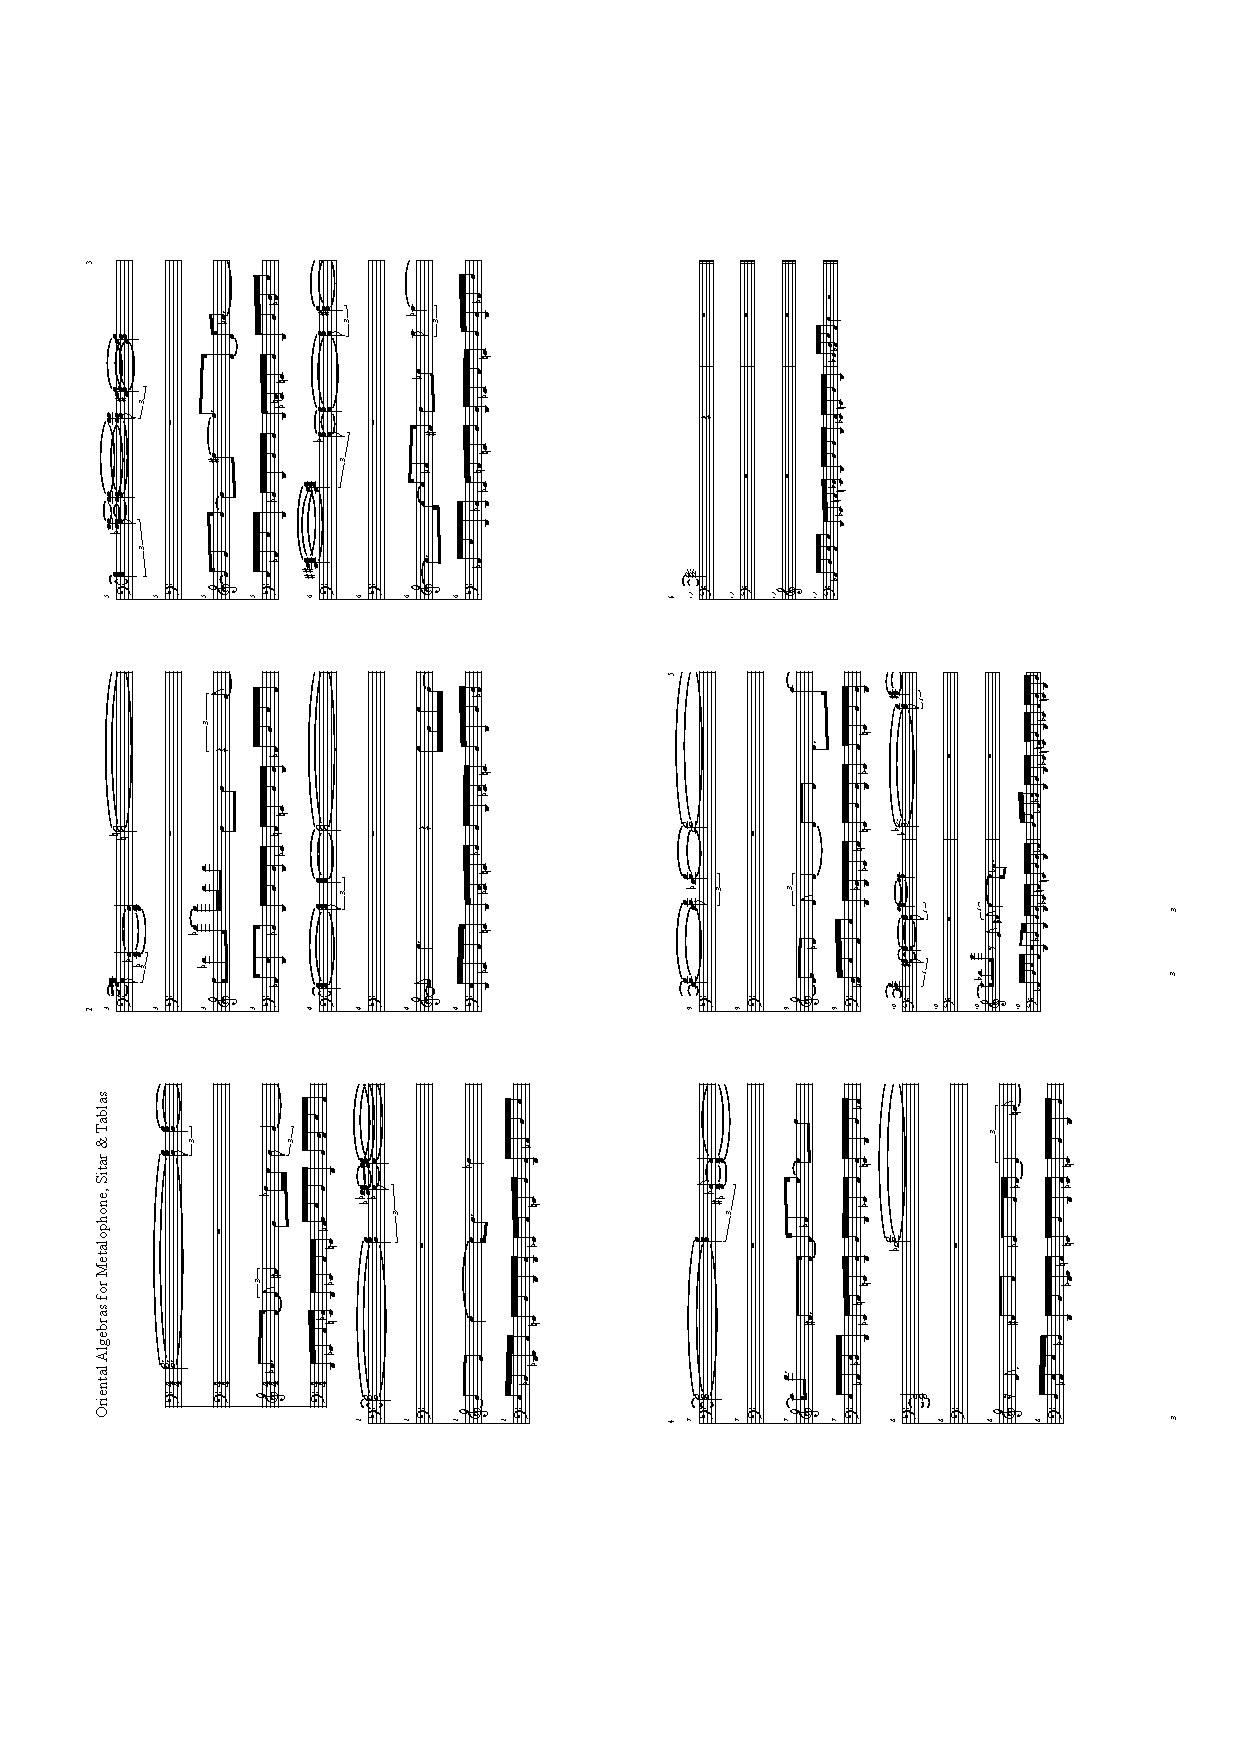
\includegraphics[width=.73\paperwidth,angle=-90]{oriental.pdf}}
    \end{center}
	\end{frame}
  	
\end{document}
 